\documentclass{article}

\usepackage[margin=1in]{geometry}

% ToC
\usepackage{blindtext} 
\usepackage[linktocpage]{hyperref}
\usepackage{bookmark}
\usepackage{titlesec}

% bib
\usepackage[round]{natbib}

% Math Imports
\usepackage{amsmath, amssymb, bm, fancyhdr, sectsty, dsfont, mathtools}

% Tikz
\usepackage{tikz}
\usetikzlibrary{bayesnet}

\usepackage{wrapfig}
\usepackage{comment}
\usepackage{subcaption}

% Symbols
\newcommand\ind{\protect\mathpalette{\protect\independenT}{\perp}}
\def\independenT#1#2{\mathrel{\rlap{$#1#2$}\mkern2mu{#1#2}}}
\newcommand\norm[1]{\left\lVert#1\right\rVert}
\newcommand\set[1]{\left\{#1\right\}}

\newcommand\RNN{\mathrm{RNN}}
\newcommand\MLP{\mathrm{MLP}}
\newcommand\enc{\mathrm{enc}}
\newcommand\softmax{\mathrm{softmax}}

% Distributions
\newcommand{\Cat}{\mathrm{Cat}}
\newcommand\Expo{\mathrm{Expo}}
\newcommand\Bern{\mathrm{Bern}}
\newcommand\Pois{\mathrm{Pois}}
\newcommand\Bin{\mathrm{Bin}}
\newcommand\Unif{\mathrm{Unif}}
\newcommand\Betad{\mathrm{Beta}}
\newcommand\Gammad{\mathrm{Gamma}}
\newcommand\Geom{\mathrm{Geom}}
\newcommand\Logd{\mathrm{Logistic}}

\newcommand\E[1]{\mathbb{E}\left[#1\right]}
\newcommand\Es[2]{\mathbb{E}_{#1}\left[#2\right]}
\newcommand{\Var}{\mathrm{Var}}
\newcommand{\Cov}{\mathrm{Cov}}
\newcommand{\Cor}{\mathrm{Cor}}

% Bold stuff
\newcommand{\ba}{\mathbf{a}}
\newcommand{\bb}{\mathbf{b}}
\newcommand{\bc}{\mathbf{c}}
\newcommand{\bd}{\mathbf{d}}
\newcommand{\be}{\mathbf{e}}
\newcommand{\bg}{\mathbf{g}}
\newcommand{\bh}{\mathbf{h}}
\newcommand{\br}{\mathbf{r}}
\newcommand{\bs}{\mathbf{s}}
\newcommand{\bw}{\mathbf{w}}
\newcommand{\bx}{\mathbf{x}}
\newcommand{\by}{\mathbf{y}}
\newcommand{\bz}{\mathbf{z}}

% mathcal stuff
\newcommand{\mcD}{\mathcal{D}}

% math blackboard bold stuff
\newcommand{\R}{\mathbb{R}}
\newcommand{\C}{\mathbb{C}}
\newcommand{\Z}{\mathbb{Z}}
\newcommand{\N}{\mathbb{N}}
\newcommand{\Q}{\mathbb{Q}}


\DeclareMathOperator*{\argmin}{argmin}
\DeclareMathOperator*{\argmax}{argmax}

\title{Latent Data to Document}

\begin{document}
\maketitle

\section{Introduction}
Neural network-based language models have achieved top performance
\citep{yang2017moslm},
allowing text generation models to become proficient at
generating short snippets of fluent text in applications such as translation \citep{bahdanau2014mt}.
Recent work in language generation has largely relied on the strong language modeling capabilities
of neural models \citep{wiseman2017d2t},
while slowly returning to the modularity afforded by probabilistic models \citep{wiseman2018template,
deng2018vattn}.
However, in leveraging powerful language models,
the field's focus has shifted from information extraction to generation as the (conditional)
language modeling capabilities of neural networks have allowed models to learn fluency.

Goals:\citet{wiseman2017d2t}, \citep{liang2009semalign}
\begin{itemize}
\item If we remove burden from the language model, will it lie less?
Only have the LM focus on fluency
\item Having a more structured model paves the way for more interpretable and
modular additions to the system, such as numerical comparisons or list modules
\end{itemize}

% Maybe goal is to demonstrate the modularity of probabilistic models?
% Need to also compare to soft model
% Result might just be that it present a different inductive bias

We would like to incorporate the modularity of a probabilistic framework into the powerful 
autoregressive modeling capabilities of a neural language model.
Although the approach brought only marginal benefits in \citet{deng2018vattn},
it can potentially be applied in many other domains. 
Alignment in translation allows models to properly condition on the source.

% Concerned with jointly learning a generative model and information extraction system.
% Is there an efficiency gain in using the approximate posterior as
% a separate system rather than finding viterbi best alignments?

\section{Problem}
We would like to learn a conditional model
over sentences $\by = \{y_0, y_1, \ldots\}$ and latent structure $\bz$ given a table $\bx$.
We are primarily interested in the respective conditional distributions:
both the posterior distribution over structure given a sentence and table $p(\bz\mid\by,\bx)$,
as well as the conditional distribution over summaries
$p(\by\mid\bx)=\Es{\bz\sim p(\bz\mid\bx)}{p(\by\mid\bz,\bx)}$.
Note that the posterior distribution over structure $p(\bz\mid\by,\bx)$
is an information extraction model.

\section{Related Work}
\citet{wiseman2017d2t}
\citet{rabinovich17codegen}
\citet{yarats2017dialogue}
\citet{liang2009semalign} also use a conditional model of utterances
and use a similar model of alignment.
However, their model is more concerned with using the posterior for information extraction and 
alignment with a database rather than both text generation as it does not include a language model. 
Instead the words are modeled independently from each other given the underlying record structure.

\section{Data to Document}
The copy models in \citet{wiseman2017d2t} are trained independently from the
information extraction model. 
The copy model is trained by generating the summary conditioned on the full table.
The information extraction model used for evaluation is trained using labels
created by comparing tokens in the summary with the entities and values from the database.
See \citet{wiseman2017d2t} for all the tricks used in training the model.

Our goal is to use more structure in our model in order to unburden the language model
and prevent hallucination of facts.

We assume that every sentence has an implicit labelling or cluster.

\subsection{The Model}
Let $y_t$ be the current token, $\by_{0:t-1}$ all previous tokens,

\begin{figure}[ht]
\centering
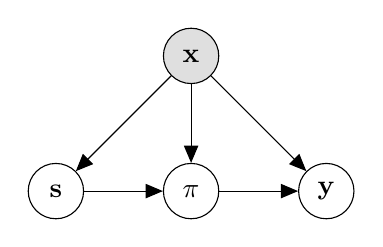
\begin{tikzpicture}
\node(x)[obs]{$\bx$};
\node(pi)[latent, below =of x]{$\pi$};
\node(s)[latent, left =of pi]{$\bs$};
\node(y)[latent, right =of pi]{$\by$};

\edge {x} {s};
\edge {x} {pi};
\edge {x} {y};
\edge {s} {pi};
\edge {pi} {y};

\end{tikzpicture}
\label{fig:dgm}
\caption{Directed graphical models for the two simplest latent variable models.
The observed context is $\tilde\bx$, current attention $a_t$, previous attention $a_{t-1}$,
state $s_t$, and target word $y_t$.}
\end{figure}

\begin{figure}[ht]
\centering
\begin{tikzpicture}
\node(x)[obs]{$\bx$};
\node(r)[latent, below =of x]{$\br$};
\node(c)[latent, left =of pi]{$\bc$};
\node(y)[latent, right =of pi]{$\by$};

\edge {x} {c};
\edge {x} {pi};
\edge {x} {y};
\edge {c} {r};
\edge {c} {y};
\edge {r} {y};

\end{tikzpicture}
\label{fig:dgm}
\caption{Directed graphical models for the two simplest latent variable models.
The observed context is $\tilde\bx$, current attention $a_t$, previous attention $a_{t-1}$,
state $s_t$, and target word $y_t$.}
\end{figure}

\section{Generative Model}
We present two conditional models, both extensions of \citet{liang2009semalign}'s
simple model that incorporate a neural language model.
We decompose structure into content selection and ordering respectively: $\bz = \set{\bs, \pi}$.

\section{Bottom-up Generative Model}
\subsection{Content Selection}
We define a distribution over records $p(\bs\mid\bx)$ where
$\bs\in\set{0,1}^n$ represents the set of binary masks over records in $\bx$.

\subsection{Record HSMM}
We can model the alignment of records to segments of text with a hidden semi-markov model (HSMM)
$p(\by,\br\mid\bs,\bx)$, similar to \citet{liang2009semalign} model.
However, we instead model the observations $\by$ with a fully-connected model,
with dependencies in-between segments.


\subsection{Permutation-Based Record Model}
Alternatively, we could 
\begin{description}
\item[Content Selection]
If a mask value is 1 then that specific relation is used to produce 
a summary.
\item[Content Ordering]
$p(\pi\mid\bs,\bx)$, where $\pi$ is a permutation matrix.
We may model this implicitly with a language model over relations, i.e. debagging.
Error: we may have repeated records.
It may be possible that certain records are only referred to a single time
while we should be available for use multiple times.
\item[Relation Realization]
$p(\by\mid\pi(\bs),\bx) = \prod_t p(y_t\mid\by_{<t}\pi(\bs)[t],\bx))$.
\end{description}

\section{Hierarchical Generative Model}
It may be better to simply use an autoregressive model of the hidden state.
\begin{description}
\item[Segment Type]
We start with a markov model $p(c_t\mid \bc_{t-1}, \bx)$
$p(c_t\mid \bc_{<t}, \bx)$
\item[Record LM]
$p(r_{t,i}\mid\br_{t,<i},c_t,\bx)$
\item[Token LM]
$p(y_{t,i,j})\mid\by_{t,i,<j},\by_{t,<i},r_{t,i})$
\end{description}

\section{Information Extraction Model}
Recall the information extraction model from \citet{wiseman2017d2t}.
$q$

\subsection{Table Completions: Learning Conjunctions}
Introduce latent variables $\bh_i\sim\Bern(\theta_i),i\in\set{0,\ldots,K}$
where $K$ is a hyperparameter. 

\subsection{Noisy Channel?}
Introduce latent variable $\bh$ and 

\section{Training and Inference}
To start, we let $q(\bz\mid\\by,\bx)$ take the form of a
delta function take the form of a segmentation.
$$q(z_t\mid\by,\bx)=$$
\subsection{Approximate Posterior or Posterior Regularization?}

\section{Related Work}

\section{Results}

\bibliographystyle{plainnat}
\bibliography{w}

\end{document}

